\documentclass[12pt]{article}
\usepackage[T1]{fontenc}
\usepackage[utf8x]{inputenc}
\usepackage[serbian]{babel}
\usepackage{lmodern}
\usepackage{geometry}
\usepackage{subcaption}
\geometry{a4paper} 
\usepackage{graphicx} 
\renewcommand{\contentsname}{Sadržaj}
\usepackage{indentfirst}
\usepackage {listings}
\lstset{language=Python}
\usepackage{hyperref}
\begin{document}
\pagenumbering{gobble}
\clearpage
\begin{figure}\begin{center}

\includegraphics[scale=0.6]{PMF.jpg}	

\includegraphics[scale=0.4]{uns.jpg}
\end{center}
\end{figure}
\begin{center}
{\huge Univerzitet u Novom Sadu \\ \ Prirodno-Matematički Fakultet, \\ \ Departman za fiziku}
\end {center}
\begin{center}
\vspace{3.cm}
 {\Huge  \textbf{Primena Python programskog jezika u meteorologiji}}
\end {center}
\begin{center}
\vspace{5.cm}
 {\large  Martin Petraš \\ \vspace{0.5cm} Novi Sad,\ 23.januar 2018}
\end {center}
\newpage
\pagebreak
\begin{center}
\tableofcontents
\end{center}
\newpage
\pagebreak
\pagenumbering{arabic}
\begin{center}
\section*{Python}
\end{center}
\begin{center}
Programski jezik Python spada u programske jezike visokog nivoa. Njegova sintaksa omogućava pisanje veoma preglednih programa, brzo i lako uči. Programski jezik Python nastao je krajem devedsetih godina prošlog veka. Njegov autor je Gvido van Rosum.Uspeh Python-a se oslanja na nekoliko prednosti koje pruža kako početnicima tako i stručnjacima: Python se lako uči. Broj funkcija u samom jeziku je skroman, pa zahteva relativno malo uloženog vremena ili napora da se naprave prvi programi. Pythonova sintaksa je dizajnirana da bude čitljiva i jednostavna. Ova jednostavnost čini Python idealnim nastavnim jezikom i omogućava početnicima da brzo napreduju. Programeri provode više vremena razmišljajući o problemu koji pokušavaju da reše, a manje vremena razmišljaju o kompleksnosti jezika ili dešifrujući kod koji su pisali drugi. 
Najosnovnije korišćenje Pythona je kao jezik skriptovanja i automatizacije, koristi se za nauku o podacima i mašinsko učenje, za veb usluge, metaprogramiranje. Njegova popularnost se ogleda u velikom broju biblioteka. Što se tiče nedostataka istakli bi njegovu brzinu. Ono za što Pythonu treba šest sekundi u drugom programskom jeziku se može uraditi za delić sekunde. Međutim, brzina kojom se može napisati funkcionalan program je daleko brži nego u nekom drugom jeziku.  
\end{center}
\newpage
\begin{center}
\section*{Uvod}
U ovom radu biće predstavljeno kako uz pomoć Pythona i njegove biblioteke Metpy možemo nacrtati polje temperature. Konkretno će obrađenja oblast u području planina Karpati. Biće pokazano kako instalirati odgovarajuće biblioteke potrebene za rad. Osvrnućemo se i na postupak interpolacije koji je korišćen kod metpy biblioteke. Prvi deo rada obuhvatiće postupke za konfigurisanje a u drugom delu će biti predstavljeni rezultati. 
\end{center}
\newpage
\section{Postupak za instaliranje}
Ovde će biti prikazan postupak instaliranja paketa potrebnih za rad u linux operativnom sistemu. 
\subsection{Provera verzije pythona}
Prvo proveravamo da li imamo instaliran python kucanjem sledeće komande:
\begin{lstlisting}
$ python 
\end{lstlisting}
Ukoliko je python instaliran pojavi se sledeće
\begin{figure}[h!]
\centering
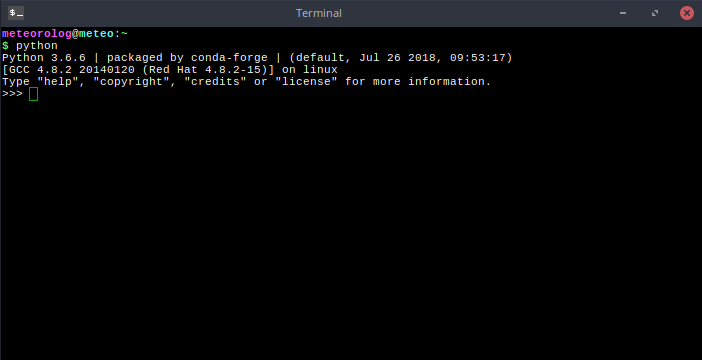
\includegraphics[width=1.\linewidth]{python.png}
\caption*{\textsl{Slika 1. Pokretanje pythona}}
\end{figure}
Uglavnom sve distribucije linuxa dolaze sa instaliranim pythonom, razlika može biti u verziji. Postoje dve verzije pythona, 2.7 čija podrška polako prestaje i novija 3.x (trenutna je 3.6.6). Razlike između ove dve verzije postoje, ali metpy biblioteka koja nama je potrebna podržava obe verzije. Više o razlikama između ove dve verzije pogledajte na \url{https://wiki.python.org/moin/Python2orPython3}. Koja verzija pythona je instalirana možemo proveriti i kucanjem sledećeg koda u terminal:
\begin{lstlisting}
$ python --version
Python 3.6.6
\end{lstlisting}  
U buduće svaki kod će biti vezan za ovu verziju.
\subsection{Izbegavanje problema sa dve verzije}
Kao što sam već spomenuo sve linux distribucija dolaze sa instaliranim pythonom, razlike mogu biti u verziji. Ukoliko vaša linux distribucija ima instaliranu samo verziju 2.7 a vi bi hteli i verziju 3.x, onda treba obratiti pažnju na sledeće. Kod mene, ja koristim MX linux distribuciju baziranu na Debian(stable) verziji, kucanjem u terminalu:
\begin{lstlisting}
$ python --version
Python 3.6.6
\end{lstlisting}  
\begin{figure}[h!]
\centering
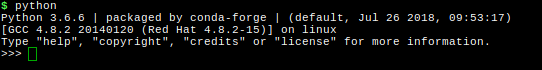
\includegraphics[width=1.\linewidth]{python3.png}
\caption*{\textsl{Slika 2. Pokretanje pythona verzije 3.6.6}}
\end{figure}
prikazuje da je podrazumevana verzija 3.6. Međutim, ukoliko je kod vas instalirana samo verzija 2.7 a vi dodatno instalirante verziju 3.x, može se desiti da će verzija 2.7 i dalje ostati podrazumevana, pa se prilikom kompajliranja može javiti problem. Pošto su kod mene obe vezije, kao podrazumevana verzija je 3.6.6 dok je za pozivanje verzije 2.7 potrebno kucati sledeće:
\begin{lstlisting}
$ python2 --version
Python 2.7.13
\end{lstlisting}
\begin{figure}[h!]
\centering
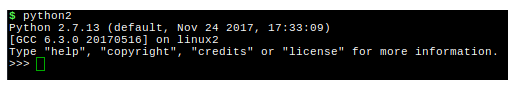
\includegraphics[width=1.\linewidth]{python2.png}
\caption*{\textsl{Slika 1. Pokretanje pythona verzije 2.7}}
\end{figure}
  Kako bi otklonili ovaj problem, u direktorijumu \textsl{/home/user/.bashrc}, koristeći jedna od tekst editora, upišemo sledeću komandu:
\begin{lstlisting}
alias python=python3
\end{lstlisting}  
Ovom komandom prilikom svakog pozivanja pythona iz terminala kao podrazumevana verzija će biti 3.6.6, što će biti jako bitno u daljem radu.
\subsection{Korišćenje modula}
Mnoge python funkcije su sadržane u specijalizovanim bibliotekama, tzv. modulima. Kako bi se ove funkcije mogle koristiti, one se moraju učitati. Učitavanje modula se postiže naredbom \textsl{import}. 





\end{document}




